\chapter{基于树形条件随机场的高阶依存句法分析}\label{cha:dep-crf}

本章深入详细的比较了与当前最佳的Biaffine Parser所采用的局部训练相比,基于全局树形条件随机场训练的方法的效果,并首次提出了在神经依存句法分析器上应用一个二阶树形条件随机场的拓展.
由于高复杂度和低效一直以来都是困扰树形条件随机场的广泛应用的一个重要原因,因此我们提出了一个能够高效批次化Inside算法和Eisner算法的方法,来支持树形条件随机场在GPU上的大规模张量并行计算.
并且,我们还通过反向传播机制,避免了复杂Outside算法的计算.
我们在13个语言的27个数据集上进行了实验,实验结果和分析表明,在深度学习时代之前的技术,诸如结构化学习(全局树形条件随机场损失函数)和高阶建模仍然是有益的,并且可以进一步在最好的Biaffine Parser的基础上提升性能,尤其是在局部标注的场景下.

\section{引言}
\begin{figure}[tb]
  \begin{center}
    \begin{dependency}%[arc edge, arc angle=80, text only label, label style={above}] %, hide label]
      %\begin{dependency} %[arc edge, arc angle=80] %, text only label, label style={above}] %, hide label]
      \begin{deptext}[column sep=.2cm] %[row sep=0.4cm, column sep=.22cm] %column sep=.2cm,
        \$$_0$ \& I$_1$ \& saw$_2$ \& Sarah$_3$ \& with$_4$ \&a$_5$ \& telescope$_6$ \\
        %\textsl{Gap:} \& $0.9$ \& $0.5$ \& $0.7$ \&[.4cm] $0.1$ \& $0.9$ \& $0.8$ \\
      \end{deptext}
      \depedge[edge style={black}]{3}{2}{nsubj}
      \depedge[edge style={black}]{3}{4}{dobj}
      \depedge[edge style={black}]{5}{7}{pobj}
      \depedge[edge style={black}]{7}{6}{det}
      \depedge[edge style={draw={rgb,255:red,76; green,114; blue,176}, thick}, label style={draw={rgb,255:red,76; green,114; blue,176}, text={rgb,255:red,76; green,114; blue,176}, semithick}]{1}{3}{root}
      \depedge[edge style={draw={rgb,255:red,76; green,114; blue,176}, thick}, label style={draw={rgb,255:red,76; green,114; blue,176}, text={rgb,255:red,76; green,114; blue,176}, semithick}]{3}{5}{prep}
    \end{dependency}
    \caption{
      一个完整依存树的例子.
      对于局部标注的场景,仅有一部分的弧被标注,例如图中两个粗蓝弧.
    }
    \label{fig:dep-tree-example} %
  \end{center}
\end{figure} %
依存句法分析任务是NLP领域的一个基础性任务,由于其简洁性,以及可以方便的在多语言上获得句法和语义信息的特性,目前在这一任务上已经有了大量的研究. 如图\ref{fig:dep-tree-example}所示,给定一个句子$\boldsymbol{x}=w_0w_1\cdots w_n$,一棵依存树被定义为$\boldsymbol{y}=\{(i\rightarrow j,l)\mid 0\le i \le n,1 \le j \le n,l \in \mathcal{L}\}$,其中$(i\rightarrow j,l)$是一条从头(head)$w_i$到修饰词(modifier)$w_j$的弧,弧的标签为$l \in \mathcal{L}$. 目前在依存句法分析任务上有两个主流方法,分别是基于转移(transition-based)的方法,和基于图(graph-based)的方法,这里我们的方法主要关注于基于图的解析方式.

在深度学习时代之前,基于图的解析依赖于很多手工特征的设计,比如词性、前缀、后缀等等.
与神经网络方法相比,以前的方法有两个显著的不同.
首先,对于非神经网络方法而言,结构化学习(结构化学习)是不可或缺的,即训练时需要显式地建模树结构的约束.
通常此类方法采用的是Max Margin训练算法,首先用当前模型训练一棵分值最高的树,然后更新模型参数,以保证正确的树的分值要高于预测树.

第二个显著的区别在于高阶特征的使用. 高阶特征为模型带来了显著的提升.
基础的一阶模型将句法树的分值分解为若干条独立的弧的分值\citep{mcdonald-etal-2005-online}. 后续的工作进一步引入了二阶依存弧对对分值,比如邻接兄弟\citep{mcdonald-pereira-2006-online}和祖父-父亲-孩子这样的弧对\citep{carreras-2007-experiments,koo-collins-2010-efficient},这些高阶扩展都带来了模型性能的显著提升\footnote{三阶和四阶模型的提升不大,这可能是由于特征稀疏的问题导致的\citep{koo-collins-2010-efficient,ma-zhao-2012-fourth}.}. 但是这些高阶模型需要引入更复杂的解码算法,导致了模型更加低效.


相比之下,基于图的神经网络依存句法分析器的发展呈现出相反的趋势.
\citep{pei-etal-2015-effective}提出利用前馈神经网络来自动学习\citep{chen-manning-2014-fast}的若干特征组合,并计算子树得分.
他们的工作表明引入二阶邻接兄弟子树的分值显著提高了性能.
随后,\citep{wang-chang-2016-graph}和\citep{kiperwasser-goldberg-2016-simple}都建议使用双向LSTM作为编码器和,以及在一阶模型中利用minus-feature来对单条弧打分.
这三个代表性方法都采用了全局的Max Margin方法.
\citep{dozat-etal-2017-biaffine}提出了一种强大而高效的Biaffine Parser,并在各种数据集和语言上获得了最先进的精度.
Biaffine Parser也是一阶的,通过对每个词进行局部头选择(head selection)的方式\citep{zhang-etal-2017-head},采用了更简单、更有效的非结构化训练方法.

基于这些对比,我们尝试在基于图的分析器的基础上,将前深度学习时代的一些方法与神经网络模型做一下连接.
这里要解决的\textbf{第一个问题}是:
\emph{以前的一些技术,比如结构化学习和高阶建模,能够进一步提升当前最佳的分析器Biaffine Parser的性能吗\footnote{
    尽管最近的一些工作汇报了相比Biaffin Parser更高的性能,但是都引入了一些外部资源,比如大规模语言模型的上下文词表示. 在相同网络和相同实验设置的场景下,这些工作的结果都是相近的.
  },如果可以,他们在哪些方面是有用的?}

对于结构化学习而言,相比Max Margin方法,我们采用更复杂且更不常用的TreeCRF.
主要原因有两方面.
首先,概率分布估计一直是当前数据驱动的NLP方法的一个核心的问题\citep{le-zuidema-2014-inside}.
如果将分析器的输出应用到更高层的任务,一棵句法树的概率$p(\boldsymbol{y}\mid\boldsymbol{x})$比没有上下边界的分值$s (\boldsymbol{x},\boldsymbol{y})$一般而言要更加有用.
其次,边缘概率是一种理论上比较可靠的方法来评估模型输出子树的置信度,可以用于最小贝叶斯风险(MBR)解码\citep{smith-smith-2007-probabilistic},并且已经被证明了对于词级别基于局部标注句法树的主动学习(active learning)\citep{li-etal-2016-active}很有用.

尽管很有用,但是TreeCRF不如Max Margin那么流行,其中一个原因是由于inside-outside算法的高复杂度,尤其是outside算法.
据我们所知,所有现存的模型都是在CPU上运算inside-outside算法.
而由于CPU/GPU巨大的效率差异,这一低效的问题在深度学习时代变得更加严重.
这就引发了\textbf{第二个问题}:
\emph{我们是否能够批次化inside-outside算法,并且直接在GPU上进行计算?}
如果这样的话,我们就能够利用诸如PyTorch这样的高效深度学习张量库来进行计算,并且将高效的TreeCRF应用到更多的场景\citep{cai-etal-2017-crf,le-zuidema-2014-inside}.

总体而言,针对上面的两个问题,我们在本章节的贡献如下:
\begin{itemize}%[leftmargin=10pt,topsep=3pt,itemsep=1pt,partopsep=1pt]
  \item 我们第一次提出了将二阶TreeCRF应用到神经依存句法分析中.
        我们还提出了一个高效的Triaffine结构来对于二阶子树打分.
  \item 我们提出通过GPU上大规模的并行张量计算来批次化inside算法,来进行更高效的TreeCRF损失函数的计算.
        我们表明复杂的outside算法对于梯度和边缘概率的计算而言已不再必须,相应的可以用高效的反向传播代替.
  \item 我们在13个语言的27个树库上进行了实验.
        结果和分析都表明,深度学习时代的,结构化学习和高阶建模在许多方面对当前最好的Biaffine Parser仍然是有用的.
\end{itemize}

\section{基线模型}
\label{sec:dep-basic-model}

我们复现了当前最好的Biaffine Parser\citep{dozat-etal-2017-biaffine},并在两方面对其做了修改:1) 用CharLSTM代替原来的词性embedding,2) 用一阶Eisner算法\citep{eisner-2000-iwptbook}代替原来的MST算法来进行投影树解码.

\subsection{打分方法}
图~\ref{fig:dep-framework}展示了我们的打分架构,一共由四个部分组成.

\textbf{输入向量.}
第$i$个输入向量可以分为两部分:词向量,以及词$w_i$的CharLSTM表示向量.
\begin{equation}
  \label{eq:input}
  \mathbf{e}_i=\mathrm{emb}({w_i}) \oplus \mathrm{CharLSTM}(w_i)
\end{equation}
其中$\mathrm{CharLSTM}(w_i)$是由先将$w_i$输入到一个双向LSTM,然后拼接两个最后的隐向量获得\citep{lample-etal-2016-neural}.
我们发现用$\mathrm{CharLSTM}(w_i)$替换原有的词性embedding会带来稳定的提升,并且也简化了实验流程,尤其是对于多语言实验恶言,无需再用到词性标注器来额外生成输入句子的词性.

\noindent\textbf{双向LSTM编码器.}
为了编码句子级别的上下文,分析器对输入$\mathbf{e}_0 \dots \mathbf{e}_n$应用了三层双.
顶层双向LSTM的第$i$个词的输出向量被表示为$\mathbf{h}_i$.

\noindent\textbf{MLP特征提取层.}
两个共享的MLP层被应用到了$\mathbf{h}_i$上来获取相应的低维向量,通过这种方式只保留句法相关的信息
\begin{equation}
  \label{mlp-arc}
  \mathbf{r}_i^{h}; \mathbf{r}_i^{m} =\mathrm{MLP}^{h/m} \left( \mathbf{h}_i \right)
\end{equation}
其中$\mathbf{r}_i^{h}$和$\mathbf{r}_i^{m}$是词$w_i$分别作为一条弧的头和修饰词的表示.

\noindent\textbf{Biaffine打分器.}
\citep{dozat-etal-2017-biaffine}首次提出通过biaffine attention计算一条依存弧$i \rightarrow j$的分值
\begin{equation} \label{eq:biaffine}
  \mathrm{s}(i,j) =  \left[
    \begin{array}{c}
      \mathbf{r}_{j}^{m} \\
      1
    \end{array}
    \right]^\mathrm{T}
  \mathbf{W}^\textit{biaffine}  \mathbf{r}_{i}^{h}
\end{equation}
其中$\mathbf{W}^\textit{biaffine} \in \mathbb{R}^{d \times d}$.
这种计算方式在GPU上进行尤其高效.

\begin{figure}[tb]
  \centering
  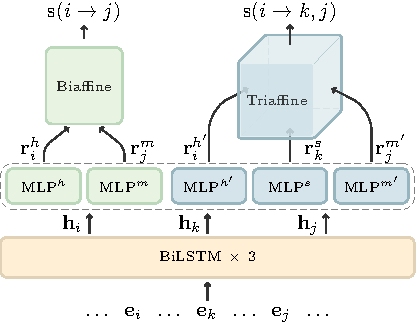
\includegraphics[scale=1.5]{figures/dep-framework.pdf}
  \caption{带二阶扩展的打分架构.}
  \label{fig:dep-framework}
\end{figure}

\subsection{局部词级别训练损失}
Biaffine Parser采用了一个简单的词级别非结构化损失函数,试着对每个词独立最大化正确头的局部概率.
在一个训练实例中,对于一个正确的头-依赖对$(w_i, w_j$),其对应的交叉熵损失为
\begin{equation} \label{eq:biaffine-loss}
  \mathit{L}(i\rightarrow j) = -\log{\frac{e^{\mathrm{s}(i\rightarrow j)}}{\sum_{0 \le k \le n} e^{\mathrm{s}(k,j)}}}
\end{equation}
换句话说,模型的训练是基于一个简单的头选择目标,最终所有词的损失都被累加起来,而没有考虑任何树结构的约束.

\subsection{解码}
有了所有依存弧的分值,我们采用复杂度为$O(n^3)$的一阶Eisner算法来寻找最优的句法树.
\begin{equation}
  \label{eq:map-decoding}
  {\boldsymbol{y}}^* = \arg\max_{\boldsymbol{y}} \left[ \mathrm{s}(\boldsymbol{x},\boldsymbol{y}) \equiv
    \sum_{i \rightarrow j \in \boldsymbol{y}}{\mathrm{s}(i\rightarrow j)} \right]
\end{equation}

\subsection{依存标签处理}\label{sub@sec:dep-crf-labeling}
Biaffine Parser将骨干树的搜索和依存弧标签标注视为两个独立的任务.
这里为了方便我们采取了相同的策略. 具体细节可以参考\citep{dozat-etal-2017-biaffine}.

\begin{figure}[tb]
  \centering
  \begin{subfigure}[b]{0.45\textwidth}
    \centering
    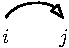
\includegraphics[scale=1.5]{figures/scoring-part/arc.pdf}
    \caption{单弧}
    \label{fig:scoring-part-arc}
  \end{subfigure}
  \begin{subfigure}[b]{0.45\textwidth}
    \centering
    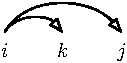
\includegraphics[scale=1.5]{figures/scoring-part/sib.pdf}
    \caption{邻接兄弟}
    \label{fig:scoring-part-sib}
  \end{subfigure}
  \caption{两种打分的子树结构.}
  \label{fig:scoring-part}
\end{figure}



\section{二阶TreeCRF}\label{2o-tree-crf}
我们从两方面极大地拓展来Biaffine Parser:
使用概率TreeCRF来进行结构化训练,以及显式引入高阶子树地分值.

具体地我们在基本的一阶模型的基础上引入了二阶邻接子树的分值:\footnote{
  我们还可以进一步扩展,引入祖父-父亲-孩子的子树分值,然后基于\citep{koo-collins-2010-efficient}提出的$O(n^4)$的Viterbi算法解码.
  这里我们留待作为未来的工作.
}
\begin{equation}\label{eq:score-definition-2o}
  \mathrm{s}(\boldsymbol{x}, \boldsymbol{y}) = \sum_{i\rightarrow j \in \boldsymbol{y}}\mathrm{s}(i\rightarrow j) + \sum_{
    %\begin{array}{c}
    i\rightarrow \{k,j\} \in \boldsymbol{y} %\
    %  i\rightarrow k \in \boldsymbol{y}
    %\end{array}
  } \mathrm{s}(i\rightarrow \{k,j\})
\end{equation}
其中$k$和$j$是$i$的两个相邻的孩子,并且满足$i < k < j$或者$j < k < i$.
图\ref{fig:scoring-part}展示了两种我们要打分的子树结构.

作为一个概率模型,TreeCRF以下面的方式计算一棵树的条件概率
\begin{equation}\label{eq:prob-labeled}
  \begin{split}
    & p(\boldsymbol{y}\mid\boldsymbol{x})  = \frac{e^{\mathrm{s}(\boldsymbol{x},\boldsymbol{y})}}{Z(\boldsymbol{x}) \equiv \sum_{\boldsymbol{y'} \in \mathcal{Y}(\boldsymbol{x})} {e^{\mathrm{s}(\boldsymbol{x},\boldsymbol{y'})}}}
  \end{split}
\end{equation}
其中$\mathcal{Y}(\boldsymbol{x})$是输入句子$\boldsymbol{x}$对应所有合法的句法树,$Z(\boldsymbol{x})$通常被成为normalization/partition term.

训练时,TreeCRF应用了下面的损失函数来最大化给定$\boldsymbol{x}$正确句法树$\boldsymbol{y}$的条件概率.
\begin{equation}\label{eq:training-loss-treecrf}
  \begin{split}
    \mathit{L}(\boldsymbol{x},\boldsymbol{y}) &= -\log p(\boldsymbol{y}\mid\boldsymbol{x})  \\
    &= - \mathrm{s}(\boldsymbol{x}, \boldsymbol{y}) + \log Z(\boldsymbol{x})
  \end{split}
\end{equation}

\begin{figure}[tb]
  \centering
  \begin{subfigure}[b]{\textwidth}
    \begin{minipage}{\textwidth}
      \centering
      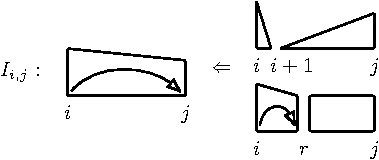
\includegraphics[scale=1.35]{figures/eisner-2o/a.pdf}
      \label{fig:eisner-2o-a}
    \end{minipage}
  \end{subfigure}
  \begin{subfigure}[b]{\textwidth}
    \begin{minipage}{\textwidth}
      \centering
      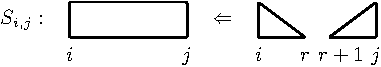
\includegraphics[scale=1.35]{figures/eisner-2o/b.pdf}
      \label{fig:eisner-2o-b}
    \end{minipage}
  \end{subfigure}
  \begin{subfigure}[b]{\textwidth}
    \begin{minipage}{\textwidth}
      \centering
      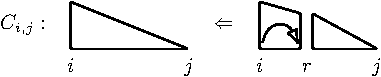
\includegraphics[scale=1.35]{figures/eisner-2o/c.pdf}
      \label{fig:eisner-2o-c}
    \end{minipage}
  \end{subfigure}
  \caption{基于自底向上动态规划的二阶Inside算法图示.}
  \label{fig:eisner-2o}
  % \vspace{-5pt}
\end{figure}

\subsection{二阶子树打分}
为了避免对原有打分架构有大的改动,我们采用来一个直接的扩展来获得邻接子树的分值.
首先,我们用三个额外的MLP层来进行和Biaffine所需要的类似的特征提取
\begin{equation}
  \label{mlp-sib}
  \mathbf{r}_i^{h'}; \mathbf{r}_i^{s}; \mathbf{r}_i^{m'} =\mathrm{MLP}^{h'/s/m'} \left( \mathbf{h}_i \right)
\end{equation}
$\mathbf{r}_i^{h'}; \mathbf{r}_i^{s}; \mathbf{r}_i^{m'}$是词$w_i$分别作为头,兄弟,和依赖对应的表示.\footnote{
  另一种方式是重用一阶部分头和依赖的表示,但是我们的前置实验表明这种方法的结果要更差一点
}

然后,我们提出来一个对biaffine equation自然的扩展,triaffine结构,来通过上述的三个向量计算分值\footnote{
  我们同样尝试了\citep{wang-etal-2019-second}的方法,他们用了三个biaffine操作来模拟三个输入向量的交互,但是这种方法的结果相对要差一点.
  篇幅限制我们省略了相应结果的汇报.
}
\begin{equation} \label{eq:triaffine}
  \mathrm{s}(i\rightarrow \{k,j\}) =
  \left[
    \begin{array}{c}
      \mathbf{r}_{k}^{s} \\
      1
    \end{array}
    \right]^\mathrm{T}
  {\mathbf{r}_{i}^{h'}}^\mathrm{T}
  \mathbf{W}^\textit{triaffine}
  \left[
    \begin{array}{c}
      \mathbf{r}_{j}^{m'} \\
      1
    \end{array}
    \right]
\end{equation}
其中$\mathbf{W}^\textit{triaffine} \in \mathbb{R}^{d' \times d' \times d'}$是一个三维的张量.
Triaffine可以方便的通过$\mathrm{einsum}$函数在GPU上高效计算.

\subsection{高效的TreeCRF计算方法}

如公式~\ref{eq:training-loss-treecrf}所示,计算TreeCRF损失的关键在于如何计算$\log Z(\boldsymbol{x})$.
这个问题在前深度学习时代的非神经网络模型上已经被很好的解决了.
我们可以在Viterbi算法的基础上,直接用sum product操作取代max product操作,这样就可以以相同的多项式时间的复杂度得到$\log Z(\boldsymbol{x})$.
然而,对非神经网络模型而言,由于缺乏自动求导机制,单独的计算Inside算法仍然是不够的.
为了获取边缘概率,然后得到特征权重的梯度,我们还需要实现更加复杂的Outside算法,而这通常要两倍慢于Inside算法.
这可能是TreeCRF在非神经网络上不如Max Margin流行的主要原因.

\begin{algorithm}[tb]
    \begin{algorithmic}[1]
        \newlength{\commentindent}
        \setlength{\commentindent}{.3\textwidth}
        \renewcommand{\algorithmiccomment}[1]{\unskip\hfill\makebox[\commentindent][l]{$\rhd$~#1}\par}
        \LetLtxMacro{\oldalgorithmic}{\algorithmic}
        \renewcommand{\algorithmic}[1][0]{
            \oldalgorithmic[#1]
            \renewcommand{\ALC@com}[1]{
                \ifnum\pdfstrcmp{##1}{default}=0\else\algorithmiccomment{##1}\fi}%
        }
        \STATE \textbf{define:} $I,S,C \in \mathbb{R}^{n \times n \times B}$ \COMMENT{$B$ is \#sents in a batch}
        \STATE \textbf{initialize:} $C_{i, i}  = 0, 0 \le i \le n$

        \FOR [span width]{$w = 1$ \TO $n$}
        \STATE \textbf{Batchify:} $0 \le i$; $j=i+w \le n$
        \STATE $I_{i, j} = \log\left(\exp\left(C_{i, i}  +  C_{j, i+1}\right) ~ +\sum\limits_{i < r < j} \exp\left(I_{i, r} + S_{r, j}+ \mathrm{s}(i, r, j)\right)\right) + \mathrm{s}(i, j)$
        \STATE $S_{i, j} = \log \sum\limits_{i \le r < j} \exp\left(C_{i, r}  +  C_{j, r+1}\right) $ \\
        \STATE $C_{i, j} = \log \sum\limits_{i < r \le j} \exp\left(I_{i, r}  +  C_{r, j}\right)  $ \\
        \ENDFOR \COMMENT{refer to Fig.~\ref{fig:eisner-2o}}
        \RETURN $C_{0, n} \equiv \log Z(\boldsymbol{x})$
    \end{algorithmic}
    \caption{二阶Inside算法.}
    \label{alg:eisner-2o}
\end{algorithm}


据我们所知,所有以前的神经网络上TreeCRF解析的工作都显式地实现了Inside-Outside算法来进行梯度的计算\citep{zhang-etal-2019-empirical, jiang-etal-2018-supervised}.
为来提升效率,这些计算通常被从GPU迁移到CPU,用Cython加速.

这里我们表明Inside算法可以被高效的批次化,从而充分利用GPU并行计算的能力.
图~\ref{fig:eisner-2o}和算法~\ref{alg:eisner-2o}展示了批次化版本的二阶Inside算法,这是\citep{mcdonald-pereira-2006-online}中的二阶Eisner算法的一个直接扩展,将其中的max product操作用sum product取代.
为了简便,我们忽略了自右边位置$j$向左边位置$i$归并生成incomplete/complete/sibling区块的描述.

具体地,对一个批次中$B$个句子,我们首先将不同位置但是相同宽度的区块($i, j$)的分值打包成为一个大的张量.
接着,我们在GPU上通过高效的大规模张量并行操作来同时进行计算和归并.
我们还可以以类似的方式来批次化解码算法,这里省略细节.

值得注意的是,这里描述的技术同样可以在其他形式的文法里应用,比如CKY算法形式的成分句法分析\citep{finkel-etal-2008-efficient,drozdov-etal-2019-unsupervised}.
具体在章节~\ref{cha:con-crf}中描述.

\subsection{Outside算法的替代:反向传播}

\citep{eisner-2016-inside}以成分句法分析(短语结构)为例,对反向传播机制和Outside算法的等价性进行了理论证明.
这里我们同样在依存句法上验证了其等价性.

进一步地,我们同样发现边缘概率$p(i \rightarrow j\mid\boldsymbol{x})$直接与对$\log Z(\boldsymbol{x})$关于分值$\mathrm{s}(i\rightarrow j)$的偏导相关
\begin{equation}
  \label{eq:dep-partial-derivative}
  \frac{\partial \log Z}{\partial \mathrm{s}(i\rightarrow j)} = p(i \rightarrow j\mid\boldsymbol{x})
\end{equation}
这可以很方便的证明(见附录~\ref{sec:outside-backprop}).
对于TreeCRF分析器,我们可以通过将解码算法中的分值用边缘概率代替,进行\textbf{最小贝叶斯风险}(Minimum Bayesian Risk, MBR)解码\citep{smith-smith-2007-probabilistic},从而带来一个稳定的提升,相关推导见附录~\ref{sec:mbr-decoding}.

\subsection{局部标注处理}
\label{sub@sec:partial-annotation}

作为一个有吸引力的研究方向,很多研究证明构建或者收集局部标注数据很有效\citep{nivre-etal-2014-squibs,hwa-99-partial-annotation,pereira-92-inside-outside},在依存句法分析中,一个句子可以关联一个局部标注树.
当结合主动学习(active learning)时,局部标注可以发挥更大的作用,由于只需要标注部分较难的子树结构,这样可以极大减轻标注者的标注负担.
\citep{li-etal-2016-active}中有关于这部分的详细调研.
此外,\citep{peng-etal-2019-overview}最近基于这方面的研究公开了一个局部标注的多领域中文树库.

那么问题就变成了如何利用局部标注数据来训练模型.
\citep{li-etal-2016-active}基于这个目的提出扩展TreeCRF到局部标注场景,并在非神经网络模型上取得了不错的效果.
这里我们借鉴他们的研究到了神经网络模型中.
我们尤其关注于在结构化学习和高阶建模上利用局部标注数据.

对基本的基于一阶局部训练方法的Biaffine Parser来说,利用局部标注最直接的方式是忽略未标注的词.
与此相对的是,树结构约束允许标注弧影响未标注词的概率分布,并且高阶建模进一步促进了词之间的交互.
因此,直觉上结构化学习和高阶建模都是非常有用的.

对于局部标注,我们和\citep{li-etal-2016-active}一样,定义训练的目标函数如下:
\begin{equation}
  \label{eq:training-loss-treecrf-partial}
  \begin{split}
    \mathit{L}(\boldsymbol{x}, {\boldsymbol{y}^p}) &= -\log \sum\limits_{\boldsymbol{y} \in \mathcal{Y}(\boldsymbol{x}); \boldsymbol{y} \supseteq {\boldsymbol{y}^p}} p(\boldsymbol{y}\mid\boldsymbol{x})  \\
    &= - \log \frac{Z(\boldsymbol{x}, {\boldsymbol{y}^p}) \equiv \sum\limits_{\boldsymbol{y} \in \mathcal{Y}(\boldsymbol{x}); \boldsymbol{y} \supseteq \boldsymbol{y}^p} e^{\mathrm{s}(\boldsymbol{x},\boldsymbol{y})}}{Z(\boldsymbol{x})}
  \end{split}
\end{equation}
其中$Z(\boldsymbol{x}, {\boldsymbol{y}^p})$ 只包含所有与给定局部标注树兼容的和法术,并且可以以与$Z(\boldsymbol{x})$类似的方式进行高效的计算.

\begin{figure}[tb]
  \centering
  \includegraphics[scale=1.2]{figures/speed.pdf}
  \caption{
    PTB的test数据上的速度比较.
  }
  \label{fig:speed}
\end{figure}

\section{实验结果及分析}\label{sec:dep-exps}
\noindent\textbf{数据.}
我们在13个语言的27个数据集上进行了实验和分析,包含两个广泛使用的数据集:英语的斯坦福依存规范\citep{chen-manning-2014-fast}的宾州树库(Penn Treebank, PTB)和中文的CoNLL09数据\citep{hajic-etal-2009-conll}.

我们还采用了公开于NLPCC19跨领域句法分析任务的中文数据集\citep{peng-etal-2019-overview},其中一共包含四个源领域和三个目标领域.
方便起见,我们直接分别合并了四个领域的Train/Dev/Test数据到更大的数据集.
这些数据的一个特征是大部分句子都是基于主动学习的局部标注.

最后,遵循\citep{ji-etal-2019-graph}和\citep{zhang-etal-2019-empirical},我们在Universal Dependencies (UD) v2.2和v2.3上进行了实验.
我们采用了\citep{zeman-etal-2018-conll}中使用的300维多语言预训练词向量,以及使用CharLSTM表示作为输入.
对于UD2.2,为了和\citep{ji-etal-2019-graph}公平比较我们和CoNLL18任务一样\citep{zeman-etal-2018-conll}使用了毛文本,并且直接使用了他们的句子分割和符号化的结果.
对于UD2.3,为了与\citep{zhang-etal-2019-empirical}比较,我们报告了使用正确词性的结果.

\begin{table}[tb!]
  \centering
  \begin{tabular}{llcccc}
    \toprule
                             &                        & \multicolumn{2}{c}{Dev} & \multicolumn{2}{c}{Test}                                                                       \\
                             &                        & UAS                     & LAS                      & UAS                              & LAS                              \\[2pt]
    \hline
    \\[-15pt]
    \multirow{10}{*}{PTB}    & Biaffine17             & -                       & -                        & 95.74                            & 94.08                            \\
                             & F\&K19                 & -                       & -                        & -                                & 91.59                            \\
    %    \cite{ma-hovy-2017-neural}        & 94.88 & 92.98 \\
    %    \cite{ma-etal-2018-stack}         & 95.87 & 94.19 \\
                             & Li19                   & 95.76                   & 93.97                    & 95.93                            & 94.19                            \\
                             & Ji19                   & 95.88                   & 93.94                    & 95.97                            & 94.31                            \\
                             & Zhang19                & -                       & -                        & -                                & 93.96                            \\[3pt]
                             & \textsc{Loc}           & 95.82                   & 93.99                    & 96.08                            & 94.47                            \\
                             & \textsc{Crf} w/o MBR   & 95.74                   & 93.96                    & 96.04                            & 94.34                            \\
                             & \textsc{Crf}           & 95.76                   & 93.99                    & 96.02                            & 94.33                            \\
                             & \textsc{Crf2o} w/o MBR & \textbf{95.92}          & \textbf{94.16}           & \textbf{96.14}                   & \textbf{94.49}                   \\
                             & \textsc{Crf2o}         & 95.90                   & 94.12                    & 96.11                            & 94.46                            \\[2pt]
    \hline
    \\[-15pt]
    \multirow{7}{*}{CoNLL09} & Biaffine17             & -                       & -                        & 88.90                            & 85.38                            \\
                             & Li19                   & 88.68                   & 85.47                    & 88.77                            & 85.58                            \\[3pt]
                             & \textsc{Loc}           & 89.07                   & 86.10                    & 89.15                            & 85.98                            \\
                             & \textsc{Crf} w/o MBR   & 89.04                   & 86.04                    & 89.14                            & 86.06                            \\
                             & \textsc{Crf}           & 89.12                   & 86.12                    & 89.28                            & 86.18\rlap{$^\dagger$}           \\
                             & \textsc{Crf2o} w/o MBR & 89.29                   & 86.24                    & 89.49                            & 86.39                            \\
                             & \textsc{Crf2o}         & \textbf{89.44}          & \textbf{86.37}           & \textbf{89.63}\rlap{$^\ddagger$} & \textbf{86.52}\rlap{$^\ddagger$} \\[2pt]
    \hline
    \\[-15pt]
    \multirow{5}{*}{NLPCC19} & \textsc{Loc}           & 77.01                   & 71.14                    & 76.92                            & 71.04                            \\
                             & \textsc{Crf} w/o MBR   & 77.40                   & 71.65                    & 77.17                            & 71.58                            \\
                             & \textsc{Crf}           & 77.34                   & 71.62                    & 77.53\rlap{$^\ddagger$}          & 71.89\rlap{$^\ddagger$}          \\
                             & \textsc{Crf2o} w/o MBR & 77.58                   & 71.92                    & 77.89                            & 72.25                            \\
                             & \textsc{Crf2o}         & \textbf{78.08}          & \textbf{72.32}           & \textbf{78.02}\rlap{$^\ddagger$} & \textbf{72.33}\rlap{$^\ddagger$} \\
    \bottomrule
  \end{tabular}
  \caption{主要结果. 我们在test上基于\textsc{Loc}做显著性检验,其中``$\dagger$''代表$\mathrm{p} < 0.05$,``$\ddagger$''代表$\mathrm{p} < 0.005$.
    Biaffine17: \cite{dozat-etal-2017-biaffine}; F\&K19: \cite{falenska-kuhn-2019-non};
    Li19: \cite{li-etal-2019-attentive}; Ji19: \cite{ji-etal-2019-graph};
    Zhang19: \cite{zhang-etal-2019-empirical}.
  }
  \label{table:dev-test}
\end{table}




\noindent\textbf{评价指标.}
我们使用无标签/有标签附着分值(UAS/LAS)作为主要的评价指标.
评价时,PTB中的词性会被忽略掉.
对于局部标注的NLPCC19数据,我们采用了官方的评价脚本,直接忽略了没有正确头标注的词.
我们采用了Dan Bikel的随机解析评价比较器来进行显著性检验.

\noindent\textbf{参数设置.}
我们直接采用了\citep{dozat-etal-2017-biaffine}的大部分参数设置,包含Dropout和初始化策略.
对于CharLSTM,和\citep{lample-etal-2016-neural}一样,输入字向量的维度是50,输出向量的维度是100.
对于二阶模型,我们设置$\mathbf{r}^{h'/s/m'}_i$的维度为100(进一步提升到300带来的提升很小).
我们训练模型最多1,000次迭代,并且如果在dev上的性能连续100次不提升那就停止训练.

\noindent\textbf{模型.}
\textsc{Loc}使用了局部交叉熵训练损失函数,并且解码时使用Eisner算法来获取最优的投影树.
\textsc{Crf}和\textsc{Crf2o}各自代表一阶和二阶TreeCRF模型.
$\textsc{Loc}_{\textsc{mst}}$代表基本的基线模型,但是解码时采用和\citep{dozat-etal-2017-biaffine}一样的MST算法输出非投影树.

\subsection{效率比较}

图~\ref{fig:speed}在PTB的测试集上比较了不同模型的解析速度.
为了能够公平比较,我们在相同的机器上运行所有的模型,模型的配置为Intel Xeon CPU (E5-2650v4, 2.20GHz)以及GeForce GTX 1080 Ti GPU.
``\textsc{Crf (cpu)}''表示直接在CPU运算Inside-Outside算法上,并利用Cython加速的模型.
由于句子间是相互独立的,因此这里还利用的多线程.
我们一共用了4个线程,并且进一步增加没有更多的提升速度.

可以看到通过批次化Inside算法以及用自动求导机制的反向传播代替Outside算法这两方面的改进,TreeCRF效率被极大的提升了.
对于\textsc{Crf}模型,我们的实现可以解析超过500句每秒,大约十倍快于多线程的``\textsc{Crf (cpu)}''.
对于二阶的\textsc{Crf2o},我们的分析器达到了400句每秒的速度,达到了实时系统的需求.

\subsection{主要结果}

表~\ref{table:dev-test}列出了Dev和Test数据上的结果.
两个数据上的结果趋势大部分是一致的.
为了能够与前人的结果公平比较,我们只比较了不利用外部资源的工作,例如ELMo\citep{peters-etal-2018-deep}或BERT\citep{devlin-etal-2019-bert}.
可以看到我们的基线模型\textsc{Loc}在PTB和CoNLL09相较于前人达到了最好的性能

在PTB上,\textsc{Crf}和\textsc{Crf2o}没有能够进一步提升解析准确率,这部分是由于这两个数据上的结果已经很高了.
然而,正如章节\ref{sub@sec:dep-analysis}所示,结构化学习和高阶建模仍然带来了一些正面的影响.

\textsc{Crf}在CoNLL09上显著超越了\textsc{Loc},并且\textsc{Crf2o}可以进一步提升性能.

在局部标注数据NLPCC19上,\textsc{Crf}极大的超过了\textsc{Loc},这表明了结构化学习在局部标注场景下的有效性.
\textsc{Crf2o}通过显式地建模二阶子树的特征,进一步的提升了解析性能.
这些结果验证了我们在章节~\ref{sub@sec:partial-annotation}的直觉性讨论.
需要注意的是,局部标注的结果看起来比较低,这里的原因是局部标注的词通常来说对于模型都是比较难的.

\subsection{分析}
\label{sub@sec:dep-analysis}

\begin{figure*}[tb!]
  \centering
  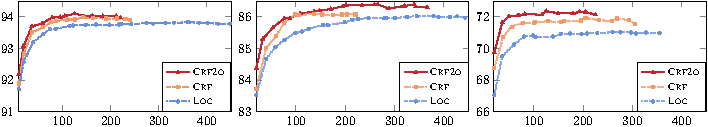
\includegraphics[width=\textwidth]{figures/convergency.pdf}
  \caption{
    PTB、CoNLL09和NLPCC19的dev数据的训练收敛曲线(LAS相对于训练迭代次数).}
  \label{fig:convergency}
\end{figure*}

\noindent\textbf{MBR解码的影响.}
对于\textsc{Crf}和\textsc{Crf2o},我们默认进行MBR解码,也就是直接在边缘概率上应用Eisner算法\citep{smith-smith-2007-probabilistic}来找到最优的句法树.
\begin{equation}
  \begin{split}
    & {\boldsymbol{y}}^* = \arg\max_{\boldsymbol{y}} \sum_{i \rightarrow j \in \boldsymbol{y}}{p(i \rightarrow j|\boldsymbol{x})}
  \end{split}
\end{equation}
表~\ref{table:dev-test}报告了MAP解码(即根据依存分值直接寻找最优句法树,关于与MBR解码的联系详见附录~\ref{sec:mbr-decoding}).
除了PTB数据集的结果已经比较高了之外,MBR解码对于\textsc{Crf}和\textsc{Crf2o}都带来了不多但是一致的提升.

\noindent\textbf{收敛行为.}
图~\ref{fig:convergency}比较了不同模型的收敛曲线.
清晰起见,我们每20次迭代选择一个结果最高的数据点放入到图里面.
可以明显看到,结构化学习和高阶建模都带来了一致的提升.
\textsc{Crf2o}稳定的达到了最好的结果,并且收敛要远远快于基本的\textsc{Loc}.

\begin{table}[tb!]
    \setlength{\tabcolsep}{5pt}
    \centering
    \begin{tabular}{llccccc}
        \toprule
                                 &                & \multicolumn{3}{c}{SIB} & \multirow{2}{*}{UCM} & \multirow{2}{*}{LCM}                                   \\
                                 &                & P                       & R                    & F                                                      \\[2pt]
        \hline
        \\[-15pt]
        \multirow{3}{*}{PTB}     & \textsc{Loc}   & 91.16                   & 90.80                & 90.98                & 61.59          & 50.66          \\
                                 & \textsc{Crf}   & 91.24                   & 90.92                & 91.08                & 61.92          & 50.33          \\
                                 & \textsc{Crf2o} & \textbf{91.56}          & \textbf{91.11}       & \textbf{91.33}       & \textbf{63.08} & \textbf{50.99} \\[2pt]
        \hline
        \\[-15pt]
        \multirow{3}{*}{CoNLL09} & \textsc{Loc}   & 79.20                   & 79.02                & 79.11                & 40.10          & 28.91          \\
                                 & \textsc{Crf}   & 79.17                   & 79.55                & 79.36                & 40.61          & 29.38          \\
                                 & \textsc{Crf2o} & \textbf{81.00}          & \textbf{80.63}       & \textbf{80.82}       & \textbf{42.53} & \textbf{30.09} \\
        \bottomrule
    \end{tabular}
    \caption{test数据上子树和完全树的结果.}
    \label{table:dev-test-subtree}
\end{table}

\noindent\textbf{子树和完全树的结果.}
除了弧级别的准确率(UAS/LAS),我们还希望能够评估模型在子树和完全树上的性能.
表~\ref{table:dev-test-subtree}展示了相关的结果.
这里我们忽略了局部标注的NLPCC19数据.
UCM(Unlabeled Complete Match)代表无标签完全匹配率,即所有对应无标签树完全正确的句子的比率,而LCM进一步要求树上的所有标签也是正确的.

对于SIB,我们评估了模型在邻接兄弟子树上的结果(系统输出和对应的正确子树).
根据公式~\ref{eq:score-definition-2o},当且仅当词$w_k$和词$w_j$都是词$w_i$的同侧孩子,并且没有其他词$w_i$的孩子在这两者之间,才称$(i,k,j)$ 是一个邻接兄弟子树.
给定两棵树,我们可以收集所有的邻接兄弟子树,然后组成一个三元组集合.
之后我们评估相应的P/R/$\mathrm{F}_1$值.
请注意在局部标注下评估SIB是做不到的.

可以明显看到,通过建模邻接兄弟子树的分值,SIB的性能相比于\textsc{Crf}和\textsc{Loc}得到了更大的提升,并且这进一步带来了进一步在完全树匹配率(UCM/LCM)上的进步.

\begin{figure}[tb!]
  \centering
  \begin{subfigure}[b]{0.4\textwidth}
    \centering
    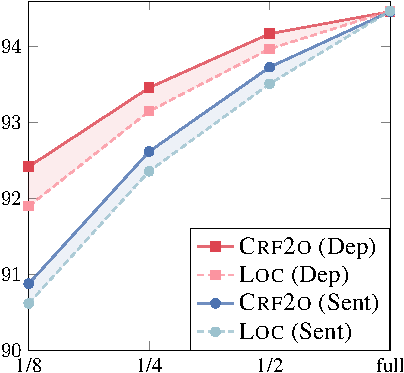
\includegraphics[width=1.\textwidth]{figures/part-gap-ptb.pdf}
  \end{subfigure}
  \begin{subfigure}[b]{0.4\textwidth}
    \centering
    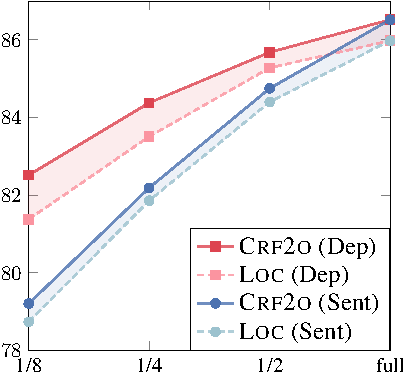
\includegraphics[width=1.\textwidth]{figures/part-gap-conll.pdf}
  \end{subfigure}
  \caption{
    PTB(左)和CoNLL09(右)的测试集有关训练数据量(弧数以及句子数)变化之后的LAS比较.
  }
  \label{fig:part-gap}
\end{figure}

\noindent\textbf{学习局部标注树的能力.}
为了更好的理解为什么\textsc{Crf2o}在局部标注的NLPCC19上表现的比较好,我们通过随机丢弃一定比例的训练数据来进行了更多的比较实验.
我们要么随机丢弃了一部分的句子(完全树),要么每个句子随机丢弃一部分弧(局部树).
图~\ref{fig:part-gap}列出了结果.

可以看到当我们渐渐地丢弃一定数量的训练句子的时候,性能差距相当稳定.
与此相反的是,当每个训练句子有更少的标注弧时,性能差距明显变得更大了.
这表明\textsc{Crf2o}在利用局部标注数据训练模型上要优于\textsc{Loc}.

\begin{table*}[tb]
    \setlength{\tabcolsep}{3.3pt}
    \centering
    \caption{UD2.2和UD2.3的test数据的LAS结果.
        同样地,$\dagger$和$\ddagger$各自表示基于\textsc{Loc}分析器,$p<0.05$以及$p<0.005$的显著性级别. }
    \begin{tabularx}{\textwidth}{lccccccccccccc}
        \toprule
                                      & bg             & ca             & cs                               & de                              & en                              & es                               & fr                              & it                               & nl                               & no                              & ro                               & ru                               & Avg.                             \\[1pt]
        \hline
        \\[-15pt]
        \multicolumn{14}{c}{UD2.2}                                                                                                                                                                                                                                                                                                                                                                                                                                   \\[1pt]
        $\textsc{Loc}_{\textsc{mst}}$ & 90.44          & 91.11          & 91.04                            & 80.21                           & 86.86                           & 90.67                            & 87.99                           & 91.19                            & 88.24                            & 90.35                           & 86.24                            & 93.01                            & 88.95                            \\
        \textsc{Loc}                  & 90.45          & 91.14          & 90.97                            & 80.02                           & 86.83                           & 90.56                            & 87.76                           & 91.14                            & 87.72                            & 90.74                           & 86.20                            & 93.01                            & 88.88                            \\
        \textsc{Crf}                  & 90.73          & 91.25          & 91.01                            & \textbf{80.56}\rlap{$^\dagger$} & 86.92                           & 90.81\rlap{$^\dagger$}           & \textbf{88.16}                  & 91.64\rlap{$^\dagger$}           & 88.10                            & 90.85                           & 86.50                            & 93.17\rlap{$^\dagger$}           & 89.14\rlap{$^\ddagger$}          \\
        \textsc{Crf2o}                & \textbf{90.77} & \textbf{91.29} & \textbf{91.54}\rlap{$^\dagger$}  & 80.46                           & \textbf{87.32}\rlap{$^\dagger$} & \textbf{90.86}\rlap{$^\dagger$}  & 87.96                           & \textbf{91.91}\rlap{$^\ddagger$} & \textbf{88.62}\rlap{$^\ddagger$} & \textbf{91.02}\rlap{$^\dagger$} & \textbf{86.90}\rlap{$^\ddagger$} & \textbf{93.33}\rlap{$^\ddagger$} & \textbf{89.33}\rlap{$^\ddagger$} \\[1pt]
        \multicolumn{14}{c}{using raw text}                                                                                                                                                                                                                                                                                                                                                                                                                          \\[1pt]
        Ji19                          & 88.28          & 89.90          & 89.85                            & 77.09                           & 81.16                           & 88.93                            & 83.73                           & 88.91                            & 84.82                            & 86.33                           & 84.44                            & 86.62                            & 85.83                            \\
        \textsc{Crf2o}                & \textbf{89.72} & \textbf{91.27} & \textbf{90.94}                   & \textbf{78.26}                  & \textbf{82.88}                  & \textbf{90.79}                   & \textbf{86.33}                  & \textbf{91.02}                   & \textbf{87.92}                   & \textbf{90.17}                  & \textbf{85.71}                   & \textbf{92.49}                   & \textbf{88.13}                   \\
        \hline
        \\[-15pt]
        \multicolumn{14}{c}{UD2.3}                                                                                                                                                                                                                                                                                                                                                                                                                                   \\[1pt]
        $\textsc{Loc}_{\textsc{mst}}$ & 90.56          & 91.03          & 91.98                            & 81.59                           & 86.83                           & 90.64                            & 88.23                           & 91.67                            & 88.20                            & 90.63                           & 86.51                            & 93.03                            & 89.23                            \\
        \textsc{Loc}                  & 90.57          & 91.10          & 91.85                            & 81.68                           & 86.54                           & 90.47                            & 88.40                           & 91.53                            & 88.18                            & 90.65                           & 86.31                            & 92.91                            & 89.19                            \\
        \textsc{Crf}                  & 90.52          & \textbf{91.19} & 92.02                            & 81.43                           & 86.88\rlap{$^\dagger$}          & 90.76\rlap{$^\dagger$}           & 88.75                           & 91.76                            & 88.08                            & \textbf{90.79}                  & 86.54                            & 93.16\rlap{$^\ddagger$}          & 89.32\rlap{$^\ddagger$}          \\
        \textsc{Crf2o}                & \textbf{90.76} & 91.12          & \textbf{92.15}\rlap{$^\ddagger$} & \textbf{81.94}                  & \textbf{86.93}\rlap{$^\dagger$} & \textbf{90.81}\rlap{$^\ddagger$} & \textbf{88.83}\rlap{$^\dagger$} & \textbf{92.34}\rlap{$^\ddagger$} & \textbf{88.21}\rlap{$^\dagger$}  & 90.78                           & \textbf{86.62}                   & \textbf{93.22}\rlap{$^\ddagger$} & \textbf{89.48}\rlap{$^\ddagger$} \\
        \multicolumn{14}{c}{using gold POS tags}                                                                                                                                                                                                                                                                                                                                                                                                                     \\[1pt]
        Zhang19                       & 90.15          & 91.39          & 91.10                            & 83.39                           & 88.52                           & 90.84                            & 88.59                           & 92.49                            & 88.37                            & 92.82                           & 84.89                            & 93.11                            & 89.85                            \\
        \textsc{Crf2o}                & \textbf{91.32} & \textbf{92.57} & \textbf{92.66}                   & \textbf{84.56}                  & \textbf{88.98}                  & \textbf{91.88}                   & \textbf{89.83}                  & \textbf{92.94}                   & \textbf{89.85}                   & \textbf{93.26}                  & \textbf{87.39}                   & \textbf{93.86}                   & \textbf{90.76}                   \\
        \bottomrule
    \end{tabularx}
    \label{table:ud-test}
\end{table*}



\subsection{UD的结果}

表~\ref{table:ud-test}比较了UD数据上不同模型的结果.
在UD数据中包含了大量的非投影树.
我们采用了\citep{nivre-nilsson-2005-pseudo}的伪投影方法来将许多语言中大量存在的非投影树转换为投影树.
基本的想法是将非投影树转换为投影树的时候利用更多更复杂的标签来标记,以方便后处理的时候能够恢复.

可以看到在基础的局部模型上,直接的基于MST算法的非投影解析方法$\textsc{Loc}_{\textsc{mst}}$和伪投影方法\textsc{Loc}达到了非常相似的性能.

更重要的是,\textsc{Crf}和\textsc{Crf2o}在大部分语言上相比于基线模型都出现了一致的提升.
在UD2.2和UD2.3上,我们提出的\textsc{Crf2o}模型在12个语言中的10个上达到了最高的解析准确率,并且在超过7个语言上获得的提升是显著的.
总体上,平均分别在UD2.2和UD2.3各自达到了0.45和0.29的提升,这同样是显著的($p<0.005$).

在UD2.2上,我们和CoNLL18任务一样采用的是毛文本,并且我们的\textsc{Crf2o}分析器上比\citep{ji-etal-2019-graph}平均要高2.30.
在UD2.3上,\citep{zhang-etal-2019-empirical}使用了正确词性作为输入,我们平均比他们高0.91.
需要注意的是\citep{ji-etal-2019-graph}里德语(de)结果错误的使用了正确的句子分割,符号化以及词性,而表中的结果是用了预测的词性,并重新运行他们的分析器得到的.
我们的\textsc{Crf2o}分析器在使用他们的词性之后平均的LAS达到了87.64.

\section{本章小结}
\label{sec:dep-conclusions}

本章首次在神经依存句法分析模型上提出了一个二阶TreeCRF的扩展,并提出使用Triaffine结构来为二阶子树打分.
我们提出了批次化的Inside算法,以适应在GPU上的并行运算.
我们同样从经验上验证了复杂的Outside算法可以隐式地通过高效的自动求导机制来完成,相应可以自然地产生梯度以及边缘概率.
我们在13个语言的27个数据集上进行了大量的实验和详尽的分析,发现结构化学习和高阶建模可以进一步地从不同的方面提升当前最佳的Biaffine Parser:1)更好的收敛行为;2)在子树和完全树上更优越的性能;3)对局部标注数据更好的利用.
